\section{Tests}

\subsection{Current test of photo diode}
This test was done in order to dimension the resistor for the operational amplifier (op-amp), for the amplification.
The desired range of the output of the amplifier is 0 to 3.3 V to make it directly correlated with the ADC, which is powered by 3.3 V. 
\subsubsection{Setup}
The photo diode is put in a breadboard and the current through is measured using a multi meter. The different colored LED's are set up with a resistor so that they draw 50 mA of current which is the max DC-current\footnote{Ref to Application note}. The LED's and the photo diode are placed as they would on the final board, with a slight tilt towards the photo diode. A brick is then held over the diodes, and the current is read off the multi meter.
The setup can be seen in figure \ref{fig:photo_diode_current_setup}.

To test if the voltage is at the expected levels, the photo diode is setup as shown in figure \ref{fig:photo_diode_voltage_setup}.

\begin{figure}[h]
 \centering
  \begin{circuitikz}
  \node[ground,name=gnd] at (0,0) {}; 
  \draw
  (gnd) to ++(0,1) to[ammeter] ++(2,0) to[pD] ++(2,0) to[R] ++(2,0)  |- (gnd)
  ;
  \draw (0,2) node[left] {$12V$} to[short, o-] ++(2,0) to[leD,mirror] ++(2,0) to[R] ++(2,0) |- (gnd); 
  \end{circuitikz}
  \caption{Setup to measure current of photo diode.}
  \label{fig:photo_diode_current_setup}
\end{figure}

\begin{figure}[h]
 \centering
  \begin{circuitikz}
  \node[op amp,name=G] at (0,0) {}; 
  \node[ground,name=gnd] at ($(G.+)+(-3,-1)$) {}; 
  \draw
  (gnd) -| (G.+) 
  (gnd) to[short] ($(G.-)+(-3,0)$) to[pD] ($(G.-)+(-0.5,0)$) node[name=intersection] {} to (G.-)
  (G.out) to ++(0,1.5) to[R] ++(-2.7,0) -| (intersection.center)
  (G.out) to[short,-o] ++(1,0) node[right,name=out] {$V_{out}$} 
  (out.west) to[voltmeter] ++(0,-1.5) -| (gnd) 
  ;
  \end{circuitikz}
  \caption{Setup to measure voltage of photo diode.}
  \label{fig:photo_diode_voltage_setup}
\end{figure}

\subsubsection{Results}
The results of the test can be seen in table \ref{tab::test_pd}.
\begin{table}[H]
\centering
 \begin{tabular}{|c|ccc|}
 \hline
 \diagbox{LED}{Brick}
        & Red         & Green       & Blue          \\ \hline
  Red   & $16\ \mu A$ & $2\ \mu A$  & $5\ \mu A$    \\ 
  Green & $5\ \mu A$  & $13\ \mu A$ & $9\ \mu A$    \\
  Blue  & $5\ \mu A$  & $6\ \mu A$  & $19\ \mu A$   \\
  \hline
 \end{tabular}
\caption{Outcome of the test}
\label{tab::test_pd}
\end{table}

Dividing $1 V$ with $10 \mu A$ in order to get the order of magnitude, gives $100 000$. This leads to the value of the resistor should be $100 000 \Omega$.
This was tested to be accurate with the setup in figure \ref{fig:photo_diode_voltage_setup}.

\subsubsection{Conclusion}
Given the results of the test, and the fact that the current used here is lower than the one used in the project\footnote{Ref to section with LED circuit} it was decided that a value of $100 000 k\Omega$ would be a reasonable. This gives $0.1 \frac{V}{\mu A}$.


\section{ADC}
To test if the ADC works with the FPGA, the ADC was tested on a breadboard.
A controlled input was given to the ADC and the MISO signal was analyzed to find the ADC value.
The ADC value is a the last 10 bits of the 17 bit package on the MISO, sent after a falling edge on the CS.
In figure \ref{fig:scope_adc} is the oscilloscope readings for a test with 2.1 V input shown.

To see how the ADC handles the input voltage a series of measurements has been made with a 0.1 V step between measurements.
In figure \ref{fig:adc_values} can the ADC values in decimal be seen in relation to the input voltage.
From this it can be seen that the ADC values are proportional to the input voltage and thus the ADC communication works.
The data code for the data processing can be found in appendix \ref{app:adc_R_code}.

\begin{figure}[h]
 \centering
 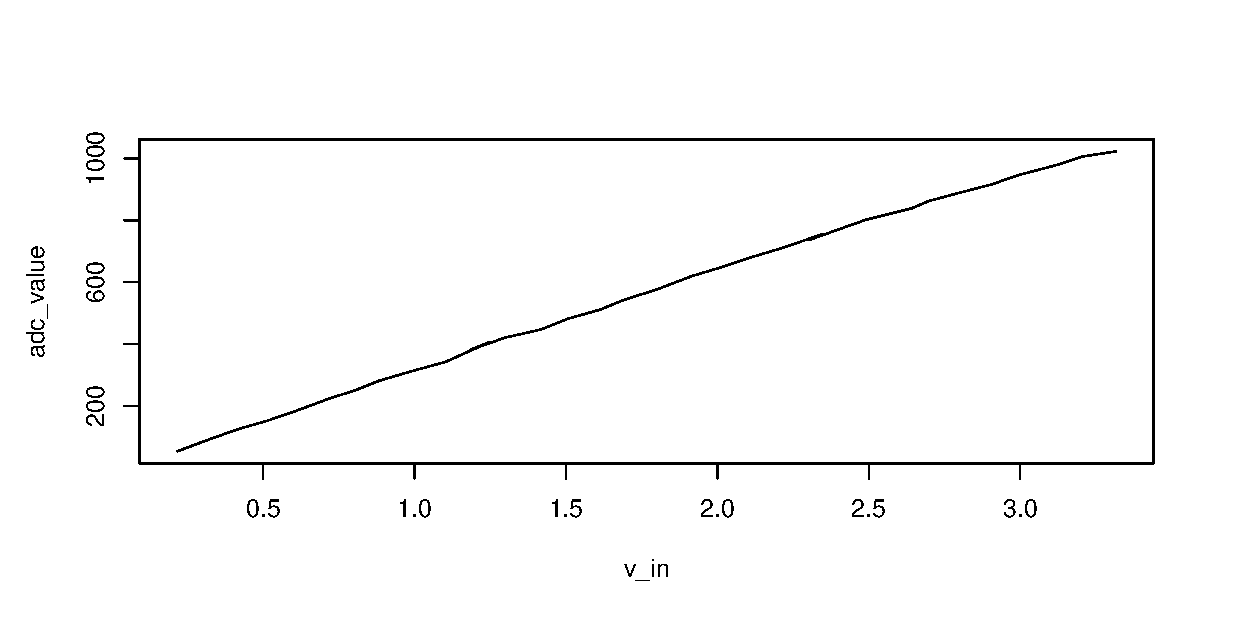
\includegraphics[width=0.7\textwidth]{img/ADC_values}
 \caption{ADC values in relation to input voltage.}
 \label{fig:adc_values}
\end{figure}

\begin{figure}[h]
    \centering
    \begin{tikzpicture}
        \node {
        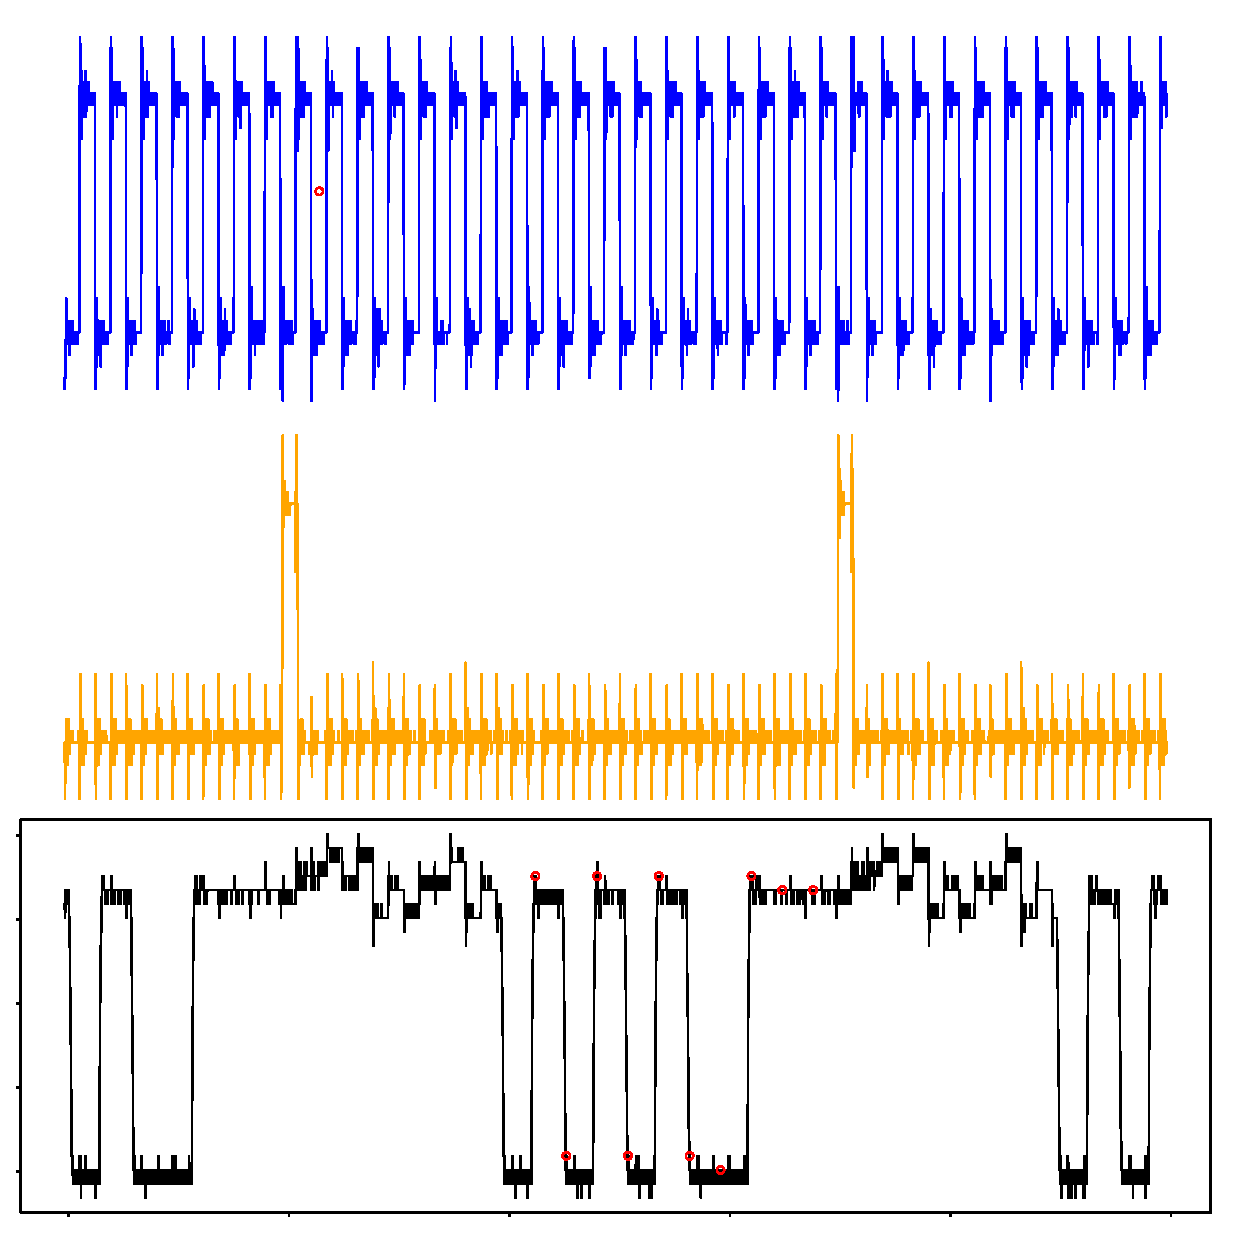
\includegraphics[width=0.7\textwidth]{img/scope_adc} 
        };
        \node at (-6.5,4)  {CLK};
        \node at (-6.5,0)  {CS};
        \node at (-6.5,-4) {MISO};
    \end{tikzpicture}
    \caption[Oscilloscope measurements for ADC]
            {Oscilloscope output of the ADC connections for the 2.107 V RMS input. The red dots signify when the signal is read.}
            \label{fig:scope_adc}
\end{figure}

